%%%%%%%%%%%%%%%%%%%%%%%%%%%%%%%%%%%%%%%%%%%%%%%%%%%%%%%%%%%%%%%%%%%%%%%%%%%%%%%%
%
% Template license:
% CC BY-NC-SA 3.0 (http://creativecommons.org/licenses/by-nc-sa/3.0/)
%
%%%%%%%%%%%%%%%%%%%%%%%%%%%%%%%%%%%%%%%%%%%%%%%%%%%%%%%%%%%%%%%%%%%%%%%%%%%%%%%%

%----------------------------------------------------------------------------------------
%	PACKAGES AND OTHER DOCUMENT CONFIGURATIONS
%----------------------------------------------------------------------------------------
\documentclass[
11pt, % The default document font size, options: 10pt, 11pt, 12pt
%oneside, % Two side (alternating margins) for binding by default, uncomment to switch to one side
%chapterinoneline,% Have the chapter title next to the number in one single line
spanish,
singlespacing, % Single line spacing, alternatives: onehalfspacing or doublespacing
%draft, % Uncomment to enable draft mode (no pictures, no links, overfull hboxes indicated)
%nolistspacing, % If the document is onehalfspacing or doublespacing, uncomment this to set spacing in lists to single
%liststotoc, % Uncomment to add the list of figures/tables/etc to the table of contents
%toctotoc, % Uncomment to add the main table of contents to the table of contents
parskip, % Uncomment to add space between paragraphs
codirector, % Uncomment to add a codirector to the title page
headsepline, % Uncomment to get a line under the header
]{MastersDoctoralThesis} % The class file specifying the document structure


%----------------------------------------------------------------------------------------
%	INFORMACIÓN DE LA MEMORIA
%----------------------------------------------------------------------------------------

\thesistitle{Equipo adquisidor de descargas parciales} % El títulos de la memoria, se usa en la carátula y se puede usar el cualquier lugar del documento con el comando \ttitle

% Nombre del posgrado, se usa en la carátula y se puede usar el cualquier lugar del documento con el comando \degreename
\posgrado{Carrera de Especialización en Sistemas Embebidos} 
%\posgrado{Carrera de Especialización en Internet de las Cosas} 
%\posgrado{Carrera de Especialización en Intelegencia Artificial}
%\posgrado{Maestría en Sistemas Embebidos} 
%\posgrado{Maestría en Internet de las cosas}

\author{Ing. Pablo Severini} % Tu nombre, se usa en la carátula y se puede usar el cualquier lugar del documento con el comando \authorname

\director{Dr. Ing. Marcos Maillot (UTN FRGP)} % El nombre del director, se usa en la carátula y se puede usar el cualquier lugar del documento con el comando \dirname
\codirector{Ing. Cristian Bonini (UTN FRGP)} % El nombre del codirector si lo hubiera, se usa en la carátula y se puede usar el cualquier lugar del documento con el comando \codirname.  Para activar este campo se debe descomentar la opción "codirector" en el comando \documentclass, línea 23.

\juradoUNO{Mg. Ing. Mara Fusco (FIUBA)} % Nombre y pertenencia del un jurado se usa en la carátula y se puede usar el cualquier lugar del documento con el comando \jur1name
\juradoDOS{Esp. Ing. Facundo Adrián Lucianna (FIUBA)} % Nombre y pertenencia del un jurado se usa en la carátula y se puede usar el cualquier lugar del documento con el comando \jur2name
\juradoTRES{Esp. Ing. Santiago Salamandri (FIUBA)} % Nombre y pertenencia del un jurado se usa en la carátula y se puede usar el cualquier lugar del documento con el comando \jur3name

%\ciudad{Ciudad Autónoma de Buenos Aires}
\ciudad{Barcelona, España}

\fechaINICIO{junio de 2020}
\fechaFINAL{junio de 2021}


\keywords{Sistemas embebidos, FIUBA} % Keywords for your thesis, print it elsewhere with \keywordnames


\usepackage[usestackEOL]{stackengine}
\def\useanchorwidth{T}
\newcommand\vstrut[1][]{\makebox[0pt]{\rule[-1ex]{1pt}{2ex}}\mnote{#1}}
\def\mnote#1{\brlap{$\scriptstyle#1$}}
\def\dx#1{\hbox to #1 {}}
\def\dline#1{\hbox to #1 {\hrulefill}}
\def\dubrace#1{\hbox to #1 {\upbracefill}}
\def\ddbrace#1{\hbox to #1 {\downbracefill}}

\begin{document}


\frontmatter % Use roman page numbering style (i, ii, iii, iv...) for the pre-content pages

\pagestyle{plain} % Default to the plain heading style until the thesis style is called for the body content


%----------------------------------------------------------------------------------------
%	RESUMEN - ABSTRACT 
%----------------------------------------------------------------------------------------

\begin{abstract}
\addchaptertocentry{\abstractname} % Add the abstract to the table of contents
%
%The Thesis Abstract is written here (and usually kept to just this page). The page is kept centered vertically so can expand into the blank space above the title too\ldots
\centering

Una Descarga Parcial (DP) es un mecanismo de ruptura dieléctrica que tiene lugar en los sistemas aislantes de máquinas y equipos eléctricos de media (MT) y alta tensión (AT). Su ocurrencia genera deterioros acumulativos en el sistema aislante que pone en riesgo sus propiedades dieléctricas, por este motivo es de interés su medición.
El presente trabajo, realizado para la UTN FRGP, trata sobre el desarrollo de un equipo para medir DP en máquinas y equipos eléctricos de MT y AT. El equipo desarrollado puede funcionar de forma autónoma y es capaz de adquirir, almacenar y procesar pulsos de DP bajo una serie de parámetros configurables. La información obtenida es utilizada para generar el Patrón de DP. Este constituye una herramienta estándar para el análisis de los sistemas aislantes de máquinas y equipos eléctricos de potencia.

\end{abstract}

%----------------------------------------------------------------------------------------
%	CONTENIDO DE LA MEMORIA  - AGRADECIMIENTOS
%----------------------------------------------------------------------------------------

\begin{acknowledgements}
%\addchaptertocentry{\acknowledgementname} % Descomentando esta línea se puede agregar los agradecimientos al índice
\vspace{1.5cm}

Esta sección es para agradecimientos personales y es totalmente \textbf{OPCIONAL}.  

\end{acknowledgements}

%----------------------------------------------------------------------------------------
%	LISTA DE CONTENIDOS/FIGURAS/TABLAS
%----------------------------------------------------------------------------------------

\tableofcontents % Prints the main table of contents

\listoffigures % Prints the list of figures

\listoftables % Prints the list of tables


%----------------------------------------------------------------------------------------
%	CONTENIDO DE LA MEMORIA  - DEDICATORIA
%----------------------------------------------------------------------------------------

\dedicatory{\textbf{Dedicado a... [OPCIONAL]}}  % escribir acá si se desea una dedicatoria

%----------------------------------------------------------------------------------------
%	CONTENIDO DE LA MEMORIA  - CAPÍTULOS
%----------------------------------------------------------------------------------------

\mainmatter % Begin numeric (1,2,3...) page numbering

\pagestyle{thesis} % Return the page headers back to the "thesis" style

% Incluir los capítulos como archivos separados desde la carpeta Chapters

% Chapter 1

\chapter{Introducción general} % Main chapter title

\label{Chapter1} % For referencing the chapter elsewhere, use \ref{Chapter1} 
\label{IntroGeneral}
En este capítulo se realiza una breve introducción de los elementos externos que interactúan con el sistema con la finalidad de brindar un marco de comprensión general antes de realizar un abordaje específico. También se explica el alcance y objetivos del presente trabajo.

%----------------------------------------------------------------------------------------

% Define some commands to keep the formatting separated from the content 
\newcommand{\keyword}[1]{\textbf{#1}}
\newcommand{\tabhead}[1]{\textbf{#1}}
\newcommand{\code}[1]{\texttt{#1}}
\newcommand{\file}[1]{\texttt{\bfseries#1}}
\newcommand{\option}[1]{\texttt{\itshape#1}}
\newcommand{\grados}{$^{\circ}$}

%----------------------------------------------------------------------------------------
%----------------------------------------------------------------------------------------
\section{Descargas parciales}
Según IEEE

\textit{(Guide for the Measurement of Partial Discharges in AC Electric Machinery)}
\enquote{Una DP es una descarga eléctrica que cortocircuita parcialmente el material aislante ubicado entre dos conductores. Cuando la tensión excede cierto valor crítico, se produce una ionización gaseosa transitoria en el sistema aislante, a dicha ionización se la denomina DP} \citep{IEEE:citation}

Una descarga parcial es un fenómeno de disrupción eléctrica. Se caracteriza por ser un pulso de corriente de alta frecuencia el cual se produce en el seno de un sistema aislante de una máquina o equipo eléctrico de potencia de media o alta tensión como consecuencia de la presencia de  oclusiones gaseosas, impurezas, aristas aguzadas u otras anomalıas que distorsionan la distribución de las líneas de campo eléctrico, figura \ref{fig:basicoDp}.

\begin{figure}[ht]
	\centering
	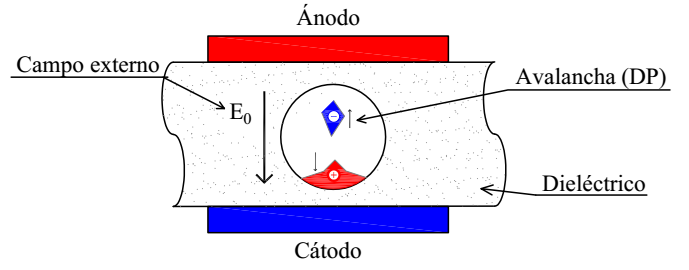
\includegraphics[width=\textwidth]{./Figures/basicoDp.png}
	\caption{Esquema básico de DP en el interior de un aislante.}
	\label{fig:basicoDp}
\end{figure}

La ocurrencia de este fenómeno provoca un deterioro del sistema aislante. Dependiendo del medio en el que este fenómeno se manifiesta y cuál sea la causa que lo origina, el deterioro del sistema puede ser acumulativo.

\section{Medidores de descargas parciales}
La técnica eléctrica más utilizada se basa en registrar las corrientes originadas por las DP en el interior del sistema aislante. La detección de estas se realiza mediante la utilización de sensores inductivos pasivos de alta frecuencia conectados en las derivaciones a tierra de los equipos que se desean ensayar.

Cuando la DP se produce en el interior del sistema aislante, las corrientes que circulan hacia tierra pasan a través del sensor inductivo; induciendo una fuerza electromotriz proporcional a la carga involucrada, figura \ref{fig:dpEjemplo}.

\begin{figure}[ht]
	\centering
	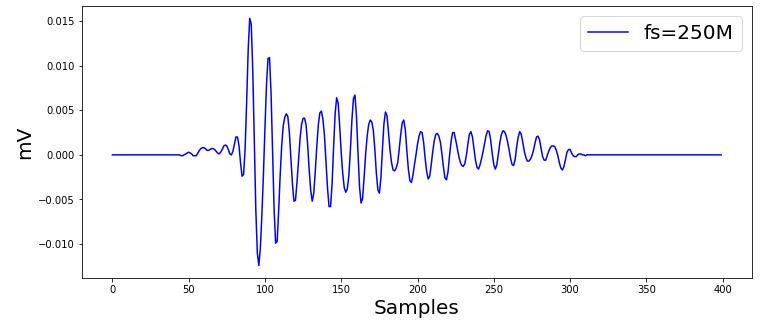
\includegraphics[width=\textwidth]{./Figures/dpEjemplo.png}
	\caption{Forma de onda de una DP capturada por un HFCT (high frequency current transformer).}
	\label{fig:dpEjemplo}
\end{figure}

Las DP registradas son representadas en un sistema de referencias en cuyo eje de ordenadas se indica la máxima amplitud del pulso y en el eje de abscisa el momento angular en que el fenómeno ocurre respecto de una senoide de referencia de 50 Hz. Por medio de la superposición de múltiples eventos sobre un mismo periodo de 50 Hz se conforma lo que se conoce en la literatura especializada como Diagrama de Magnitud - Fase o Patrón de DP, figura \ref{fig:patronEjemplo}.

\begin{figure}[!ht]
	\centering
	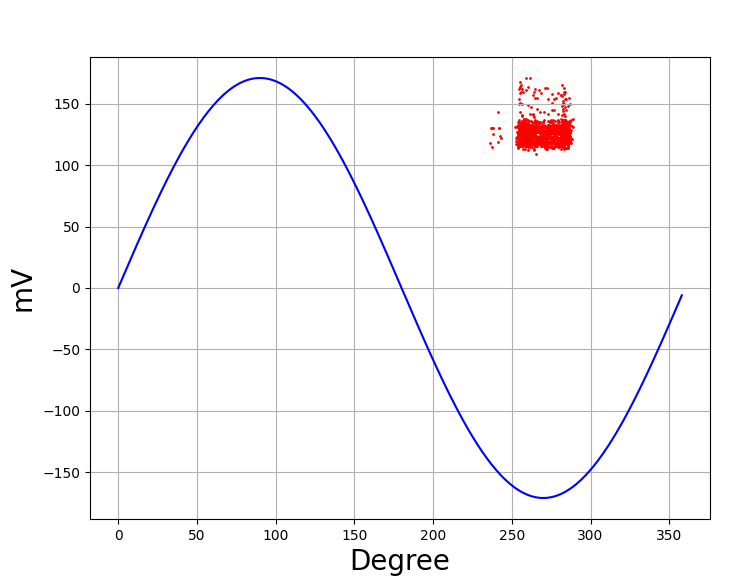
\includegraphics[width=100mm]{./Figures/patronEjemplo.png}
	\caption{Patrón de DP.}
	\label{fig:patronEjemplo}
\end{figure}

Los patrones de DP permiten identificar, por medio de su estructura, el grado de severidad de un falla \citep{Gulski:citation}. También permiten emitir un diagnóstico, ya que distintos tipos de DP tienen asociados distintos riesgos \citep{Cavallini:citation}.

Sensor inductivo

Los transformadores de corriente de alta frecuencia (HFCT), figura \ref{fig:hfct}, son sensores inductivos que dada su robustez y su sensibilidad están ampliamente difundidos como elementos captores para mediciones de DP en campo. Estos se instalan en las derivaciones a tierra de las máquinas o equipos eléctricos de potencia donde se desea medir la ocurrencia de este fenómeno.


\begin{figure}[ht]
	\centering
	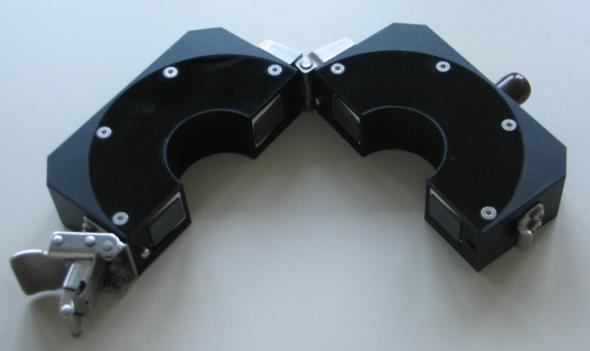
\includegraphics[width=100mm]{./Figures/hfct1.png}
	\caption{HFCT de la empresa TechImp.}
	\label{fig:hfct}
\end{figure}

\section{Estado del arte}
Actualmente existen equipos de medición de DP fabricados por empresas extranjeras como TechImp, PD Power Diagnostix u Omnicrom. Si bien esta gama de equipos abarca un amplio rango de características, ninguno proporciona una herramienta considerada de bajo costo para nuestro país, que permita a cooperativas o medianas empresas acceder a este herramienta de diagnóstico. Al mismo tiempo, este equipo proporciona una herramienta de base para implementar algoritmos propios para procesamiento \textit{over the edge}; características que no tienen los actuales equipos en el mercado. 

Equipos existentes en el mercado de características similares al equipo desarrollado:

TechImp Falcon \citep{falconWeb:1}
\begin{itemize}
\item Solución “económica” para monitoreo constante de DP.
\item Adquisición automática y generación del patrón de DP.
\item Separación de las diferentes actividades de descargas.
\item Ancho de banda 30 MHz resolución 12 bits.
\item Conexión ethernet.
\end{itemize}

\begin{figure}[h!]
	\centering
	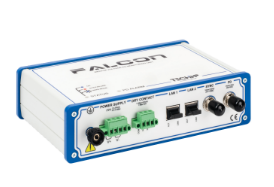
\includegraphics[width=80mm]{./Figures/arte1.png}
	\caption{Equipo Falcon de Techimp.}
	\label{fig:arte1}
\end{figure}


\vspace{15mm}
PD Power Diagnostix ICMmonitor \citep{pdWeb:1}
\begin{itemize}
\item Creación del patrón y display para visualización \textit{in-situ}.
\item Analizador de espectro.
\item Posibilidad de monitoreo remoto.
\item Conexión TCP.
\end{itemize}

\begin{figure}[h!]
	\centering
	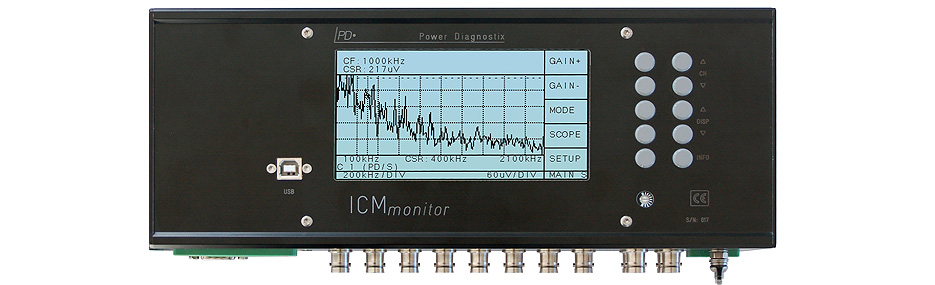
\includegraphics[width=90mm]{./Figures/arte2.png}
	\caption{Equipo ICMmonitor de PD Power Diagnostix.}
	\label{fig:arte2}
\end{figure}


Omicrom MPD600 \citep{mpdWeb:1}
\begin{itemize}
\item Medicion y analisis de descargas.
\item Permite grabar, analizar y mostrar las señales.
\end{itemize}

\begin{figure}[h!]
	\centering
	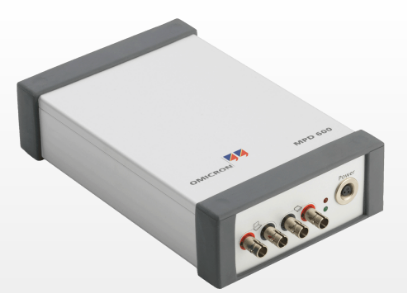
\includegraphics[width=80mm]{./Figures/arte3.png}
	\caption{MPD600 de Omnicrom.}
	\label{fig:arte3}
\end{figure}

\section{Objetivos y alcance}
\subsection{Objetivos}
El objetivo de este trabajo fue desarrollar un prototipo de un equipo adquisidor de DP de calidad, de bajo costo y de producción nacional. A su vez, se buscó crear las bases para un equipo abierto con capacidad de hacer procesamiento \textit{over the edge}. 

\subsection{Alcance}
El alcance del trabajo incluyó:
\begin{itemize}
\item El desarrollo del prototipo del producto.
\item El desarrollo del firmware.
\item El diseño del circuito esquemático.
\item Confección de un manual de uso.
\item Pruebas de validación y verificación.
\end{itemize}


\chapter{Introducción específica} % Main chapter title

\label{Chapter2}

%----------------------------------------------------------------------------------------
%	SECTION 1
%----------------------------------------------------------------------------------------
Durante este capítulo se brinda un marco orientativo sobre los requerimientos específicos del proyecto, la teoría básica involucrada y las tecnologías utilizadas para su realización.

\section{Requerimientos}
El trabajo realizado es un equipo adquisidor de DP que tiene como cliente a la UTN FRGP. 

A continuación se listan los requerimientos acordados al iniciar el trabajo. Cabe destacar que todos fueron cumplimentados en su totalidad con excepción de los requerimientos 23 y 24 que fueron modificados, de mutuo acuerdo con el cliente, sin generar deterioro alguno en las características del equipo.

\begin{itemize}
\item Req 1: El dispositivo deberá, mediante el procesamiento de las adquisiciones, detectar los picos máximos de los pulsos de DP y representarlos sobre una senoide de referencia de frecuencia industrial - 50 Hertz - en fase con la tensión de ensayo (generar un patrón de DP).
\item Req 2: El dispositivo deberá funcionar como un sistema \textit{stand-alone}.
\item Req 3: El dispositivo deberá mantener la fecha y hora por medio de un RTC.
\item Req 4: El dispositivo deberá tener un puerto de acceso serial (preferentemente diferencial) para configuración y acceso a datos remoto.
\item Req 5: El dispositivo deberá contar con un puerto USB para la descarga de los patrones de DP.
\item Req 6: El dispositivo deberá permitir modificar el umbral de disparo a partir del cual se comenzará a adquirir una señal.
\item Req 7: El dispositivo deberá permitir modificar la cantidad de muestras que serán adquiridas por disparo (máximo 1000).
\item Req 8: El dispositivo deberá permitir modificar la cantidad de disparos (máximo 1000) que componen a un patrón de DP.
\item Req 9: El dispositivo deberá permitir configurar el RTC.
\item Req 10: El dispositivo deberá permitir planificar la generación automática de un patrón DP cada periodos múltiplos de 1 hora (calendario).
\item Req 11: El dispositivo deberá permitir generar un patrón de DP con los parámetros configurados a demanda y transferirlo por el puerto serie.
\item Req 12: El dispositivo deberá permitir poner al sistema en modo “ARMADO” o “ DESARMADO”.
\item Req 13: En modo “ARMADO” el dispositivo deberá cumplir con las adquisiciones preestablecidas por calendario.
\item Req 14: En modo “DESARMADO” el dispositivo no estará operativo.
\item Req 15: La entrada de señal de referencia debe poder detectar los cruces por cero de una senoide de 50 Hz, y saber su polaridad.
\item Req 16: La entrada de señal de referencia debe ser opto-acoplada.
\item Req 17: El dispositivo deberá llevar un contador en milisegundos a partir de la señal de cruce por cero. De forma tal que se pueda saber en todo momento si está transcurriendo un semiciclo positivo o negativo y saber cuánto tiempo transcurrió desde su inicio.
\item Req 18: Se deben poder adquirir señales con una ancho de banda entre 0.1 MHz y 40 MHz con una resolución mínima de 8 bits.
\item Req 19: La amplitud máxima de la señal de entrada será de 1 Vpp.
\item Req 20: La entrada para el sensor analógico deberá ser de 50 ohms diferencial.
\item Req 21: El dispositivo deberá detectar cuando la señal muestreada supere el umbral de disparo, si esto sucediera las siguientes muestras (cantidad definida anteriormente en la configuración) deberán ser comparadas entre sí y preservar la de mayor magnitud. El valor obtenido deberá ser almacenado en memoria, junto con un timestamp, la polaridad del semiciclo de referencia y su momento angular. Este proceso debe ser repetido hasta que se cumplan los disparos que componen un patrón DP.
\item Req 22: Deberá indicará su estado “ARMADO - DESARMADO” por medio de un led de estado.
\item Req 23: Deberá permitir “ARMAR - DESARMAR” al sistema por medio de una tecla física.
\item Req 24: Deberá realizar la acción de transferir a un pendrive el contenido total de la memoria interna por medio de una tecla fısica.
\item Req 25: El dispositivo deberá listar todos los patrones de DP almacenados bajo el siguiente identificador “AAMMDDhhmm” en base a la fecha de generación del patrón.
\item Req 26: El dispositivo deberá permitir seleccionar al patrón por medio de su identificador y solicitar su transferencia por puerto serie.
\end{itemize}

Los requerimientos 23 y 24 fueron modificados debido a que el almacenamiento de las DP es realizado directamente en el pendrive. De esta forma se puede reducir el costo en el diseño y se elimina la necesidad de transferir archivos entre memorias. Ambos requerimientos fueron reemplazados por el siguiente:
\begin{itemize}
\item Deberá almacenar en el pendrive el patrón de DP al finalizar su adquisición.
\end{itemize}


\section{Descripción general del sistema}

En la figura \ref{fig:bloques} se brinda una introducción de los módulos principales que abarcan el sistema y su interacción, por medio de esta se busca brindar una mejor interpretación de algunos temas abordados en este capítulo.

\begin{figure}[ht]
	\centering
	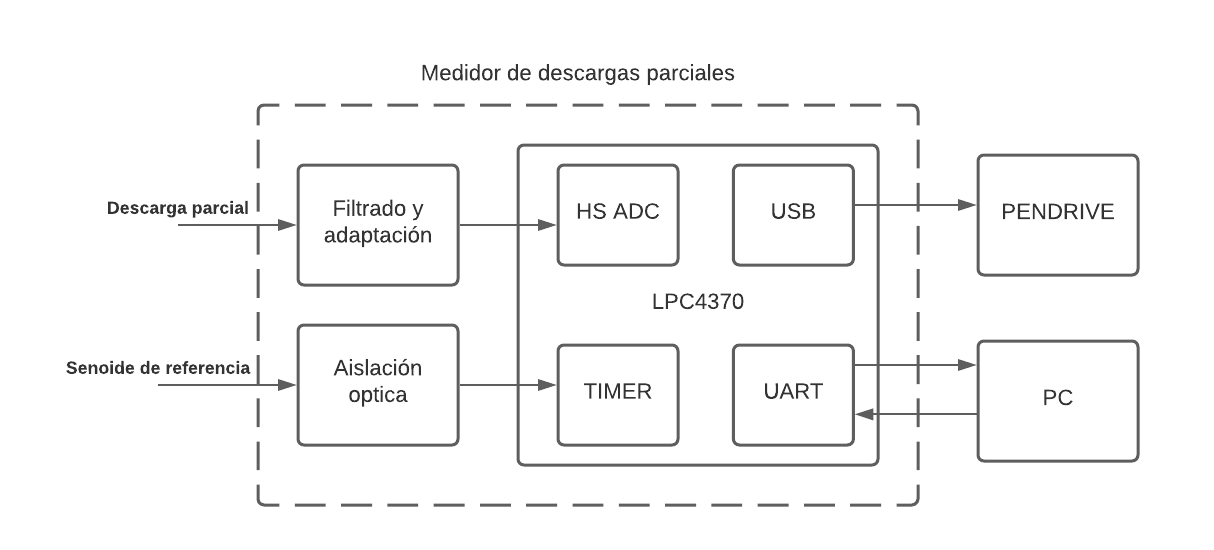
\includegraphics[width=\textwidth]{./Figures/bloques.png}
	\caption{Diagrama en bloques de sistema.}
	\label{fig:bloques}
\end{figure}

El objetivo principal del equipo consiste en adquirir, almacenar y procesar señales de DPs para posteriormente, junto a la senoide de referencia, conformar el diagrama de magnitud-fase o patrón de DP.

\section{Aislación óptica}
Un optoacoplador es un dispositivo que vincula de forma óptica un diodo led y un fototransistor a través  de material aislante transparente. Utilizados como interfaz entre circuitos con diferentes potenciales de masa, los optoacopladores reemplazan la aislación por medio de transformadores y relés. También son utilizados para aislar circuitos lógicos y líneas de potencia evitando cambios de impedancia, mejorando la capacidad de aislación entre entrada y salida y facilitando la eliminación del ruido \citep{opto:appnote}. Para este equipo se seleccionó el optoacoplador LTV357 \citep{opto:ltv357} de la empresa liteon, el mismo cumple con los requisitos de ser de bajo costo, tener una aislación de 3750 Vrms y una respuesta lineal hasta 2 KHz de frecuencia.

\begin{figure}[ht]
	\centering
	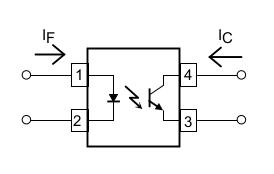
\includegraphics[width=70mm]{./Figures/opto.png}
	\caption{Representación esquemática de un optoacoplador.}
	\label{fig:opto}
\end{figure}

\section{Filtrado y adaptación}
Una etapa de filtrado y adaptación es un punto crítico para cualquier diseño de adquisición de señales analógicas. La señal proveniente de los sensores puede contener componentes de frecuencia fuera del ancho de banda de interés. También es posible que los niveles de tensión de la señal no utilicen al máximo el rango dinámico de entrada perdiendo bits de conversión. La saturación por sobretensión también es un elemento que perjudica a la calidad de las mediciones y en algunos casos puede destruir al equipo. 

La etapa de filtrado está diseñada para dejar pasar las frecuencias dentro de la banda de interés, atenuando en gran parte a todas aquellas fuera de rango.

La etapa de adaptación permite llevar los niveles de tensión de entrada al máximo rango dinámico permitido, esto puede realizarse por medio de amplificación o atenuación de la señal dependiendo el caso. En esta etapa también se implementan protecciones por sobretensión que puedan dañar al equipo, normalmente diseñadas con diodos de alta velocidad.

\section{Procesamiento}
La etapa de procesamiento es la encargada de orquestar todos los módulos del sistema. El equipo utiliza como microcontrolador principal un LPC4370 \citep{micro:lpc4370} de la firma NXP. La elección fue determinada porque posee un conversor analógico digital de alta velocidad (80 MSPS) combinado con un procesador ARM cortex M4 y dos ARM cortex M0. También incluye en la versión con encapsulado TFBGA100 dos periféricos USB de alta velocidad, puerto serie, reloj de tiempo real y entradas de propósito general.

Fue determinante para su elección el periférico ADCHS y su bajo costo. Gracias a que los principales módulos del desarrollo pudieron ser resueltos con los periféricos internos, solo fue necesario implementar de forma externa la etapa de aislación óptica y la etapa de adaptación y filtrado de señal.

Periféricos utilizados: 
\begin{itemize}

\item HS ADC - Conversor analógico digital de alta velocidad

El LPC4370 TFBGA100 dispone de 3 conversores analógicos digitales de alta velocidad. Este es un periférico complejo que permite realizar adquisiciones analógicas a una tasa de muestreo de 80 MSPS con una resolución de 12 bits. Para poder manejar este flujo de datos proporciona conexión por DMA. Otro característica importante es el sistema de disparo del trigger, que permite dos umbrales de disparo por flanco ascendente o descendente.

\item Timers

Dispone de 4 timers de 32 bits, que permiten ser configurados como contadores o temporizadores. Para permitir una mejor adaptación a los tiempos de aplicación, proporcionan divisores y diferentes opciones suministro de clock.


\item USB

Dispone de 2 puertos USB 2.0 con velocidad de transferencia de hasta 480 Mb/s. Uno de ellos con tecnología on-the-go. Ambos soportan DMA  y cumplen con las especificaciones Universal Serial Bus 2.0

\item RTC - Reloj de tiempo real

Dispone de un reloj de tiempo real con registros específicos para funcionar en bajo consumo. Este módulo requiere de un cristal propio de 32 KHz para generar una base de tiempo de 1 Hz independiente al CPU, también posee una línea de alimentación dedicada que puede ser alimentada por batería.
\end{itemize}


\section{Muestreo de datos}
Para procesar y almacenar las señales analógicas de alta frecuencia proveniente del pulso de una DP es preciso realizar un muestreo de amplitud de la señal. 

El concepto de muestreo de amplitud de una señal analógica en intervalos de tiempo discretos se muestra en la figura \ref{fig:muestreo1}.

La señal analógica debe ser muestreada en intervalos de tiempo discretos ts, este intervalo debe ser cuidadosamente escogido para asegurar una precisa representacion de la señal analógica original. Está claro que a mayor cantidad de muestras adquiridas mayor será la precisión de la representación digital, pero sí pocas muestras son tomadas se alcanza un punto en donde se pierde información crítica de la señal. Este punto está definido por los criterios de Nyquist \citep{sampling:appnote}.

\begin{figure}[ht]
	\centering
	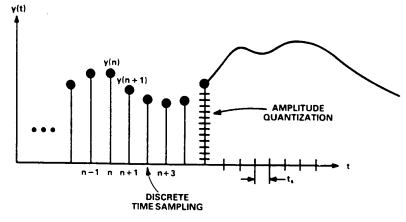
\includegraphics[width=100mm]{./Figures/muestreo1.png}
	\caption{Muestreo discreto de una señal analogica.}
	\label{fig:muestreo1}
\end{figure}

Criterios de Nyquist
\begin{itemize}
\item Una señal analógica con un ancho de banda de \textit{fa} debe ser muestrado a una tasa de muestreo \textit{fs>2fa} para evitar pérdida de información.
\item Si \textit{fs<2fa} entonces un fenómeno llamado \textit{aliasing} ocurre en el ancho de banda de la señal
\end{itemize}

Con el fin de comprender la implicación del \textit{aliasing} se deben considerar los cuatro casos representados en la figura \ref{fig:muestreo2} de una señal senoidal muestreada en el dominio del tiempo.
En el caso 1 está claro que la cantidad de muestras es adecuada para preservar la información. En el caso 2 solo se realizaron 4 muestras por ciclo, pero aun así es una cantidad adecuada para preservar la información. En el caso 3 se representa un caso de la condición límite ambiguo donde \textit{fs=2fa}. Si la relación entre los puntos muestreados y la señal fuese tal que el muestreo coincidiera con los cruces por cero, toda la información se perdería. En el caso 4 la figura representa la situación donde \textit{fs<2fa} y la información obtenida de las muestras dan como resultado una senoide de frecuencia inferior a \textit{fs/2}, en este caso una frecuencia fuera de banda se entrelazo con ancho de banda de Nyquist. 

\begin{figure}[ht]
	\centering
	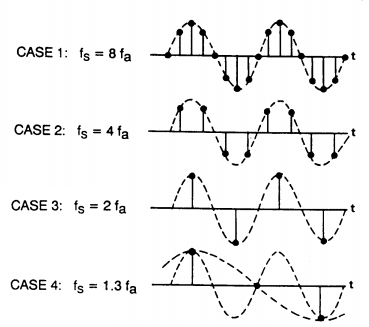
\includegraphics[width=100mm]{./Figures/muestreo2.png}
	\caption{Efecto \textit{aliasing} en señales analogicas.}
	\label{fig:muestreo2}
\end{figure}

Por lo expuesto anteriormente, un conversor analógico digital debe ser precedido por un filtro \textit{anti-aliasing}, figura \ref{fig:muestreo3}, que tenga suficiente atenuación a partir de la frecuencia de corte \textit{fs/2} para prevenir que se entrelacen frecuencias fuera de banda.

\begin{figure}[ht]
	\centering
	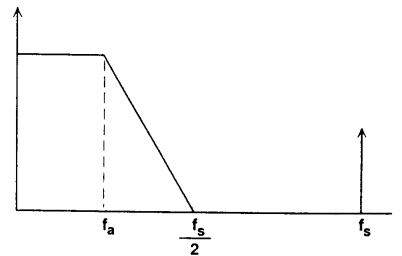
\includegraphics[width=100mm]{./Figures/muestreo3.png}
	\caption{Filtro pasabajos \textit{anti-aliasing}.}
	\label{fig:muestreo3}
\end{figure}

\section{Listado de herramientas utilizadas}
Para este trabajo se utilizaron las siguientes herramientas de hardware:
\begin{itemize}
\item Placa LPC Link2 como programador y \textit{debugger}.
\item Placa LPC Link2 como placa de desarrollo.
\item Fuente de alimentación conmutada Minileaf 0-30V 10A
\item Osciloscopio Siglent SDS1202X-E de 200 MHz para verificar las mediciones y tiempos realizados por el equipo.
\item DDS FY6900 de 60 MHz para la generación de señales en el banco de pruebas.
\item Analizador lógico Saleae para el control de tiempos.
\item Multímetro.
\end{itemize}


También se utilizaron la siguiente herramientas de software:
\begin{itemize}
\item Mcuxpresso ide 11.3 para el diseño del firmware \citep{mcuxpresso}.
\item Python 3 para la generación de scripts para el banco de prueba y scripts de procesamiento de datos.
\item Minicom para acceder a la interfaz.
\end{itemize}
 
\chapter{Diseño e implementación} % Main chapter title

\label{Chapter3} % Change X to a consecutive number; for referencing this chapter elsewhere, use \ref{ChapterX}
Durante este capítulo se realiza una explica el diseño e implementación del software y hardware del equipo. También se detalla y justifica el motivo de las implementaciones realizadas.

\section{Diseño del Hardware}
\subsection{Cruce por cero}

Debido a que la medición de una descarga parcial debe estar relacionada con la senoide de referencia por medio de su momento angular, el equipo fue provisto de un medio para conocer esta variable del sistema de forma constante.

El método elegido para la medición de fase fue un circuito de detección de cruce por cero combinado con un timer interno del microcontrolador. Se optó por este método porque puede ser aislado por medio de un optoacoplador y soportar conexiones directas con senoides de referencia de hasta 300 V. Otro motivo es que solo al ser de interés el momento angular, un timer de 32 bits brinda mejor resolución que un conversor analógico digital y requiere menos procesamiento.

El circuito diseñado, figura \ref{fig:schZeroCross}, está basado en un optocoplador LTV357 \citep{opto:ltv357}. Este presenta una aislación de 3750 Vrms entre entrada y salida. La polarización del led de entrada se realizó por medio de un C8 y tiene un rango dinámico de tensión de entrada entre 50 Vpp y 340 Vpp. 

\begin{figure}[ht]
	\centering
	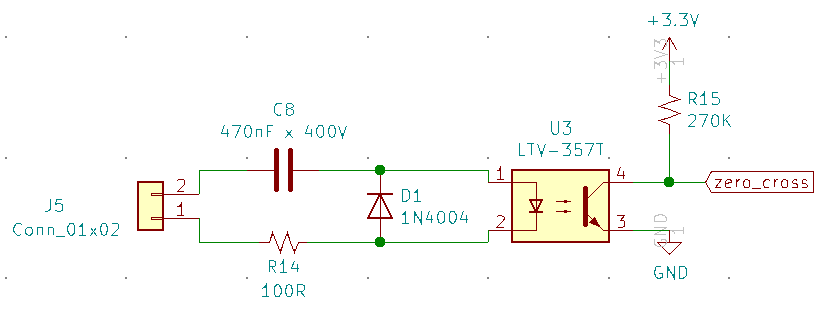
\includegraphics[width=130mm]{./Figures/schZeroCross.png}
	\caption{Entrada de detección de cruce por cero para la senoide de referencia.}
	\label{fig:schZeroCross}
\end{figure}

\newpage

El cálculo del valor de C8 fue determinado por la corriente de polarización del led (\textit{If}), la corriente de colector (\textit{Ic}) y la relación de transferencia (CTR), figura \ref{fig:ltvCtr}.  

\begin{figure}[ht]
	\centering
	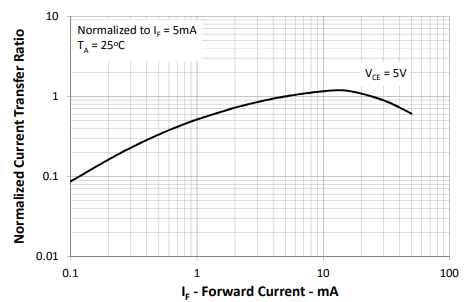
\includegraphics[width=130mm]{./Figures/ltvCtr.png}
	\caption{Relacion de transferencia del LTV357.}
	\label{fig:ltvCtr}
\end{figure}

En base a la curva \ref{fig:ltvCtr}, se calculó la corriente mínima necesaria \textit{If} para polarizar el transistor del optoacoplador. Para este cálculo se consideró como tensión mínima de polarización, a una senoide de 50 Vpp luego de haber transcurrido 1 grado desde su cruce por cero. Esto se debe a que la resolución mínima deseada del equipo es 1 grado y por lo tanto el circuito debe detectar el cruce por cero dentro de este periodo.

En la tabla \ref{tab:corriente} se observa que la corriente \textit{If} máxima en 340 Vpp no excede los 50 mA y que la corriente \textit{Ic} mínima en 50 Vpp es superior a los 0,0122 mA necesarios para polarizar el circuito.

\vspace{5mm}

\begin{table}[h]
\centering
\caption[Corrientes de polarización]{Corrientes de polarización}
\begin{tabular}{l c c c c}
\toprule
\textbf{Vpp} & \textbf{If(mA) @ 1°} & \textbf{Ic(mA) @ 1°} & \textbf{If(mA) @ 90°} & \textbf{Ic(mA) @ 90°}\\
\midrule
340 & 0,88 & 0,35 & 50,2 & 30,12 \\
50 & 0,13 & 0,0129 & 7,38 & 7,38\\
\bottomrule
\hline
\end{tabular}
\label{tab:corriente}
\end{table}

\vspace{5mm}

El optoacoplador elegido solo posee un led, por lo que se polariza durante un semiciclo esto permite reconocer de forma sencilla el semiciclo positivo y negativo. El diodo D1 protege al diodo interno del optoacoplador cuando se encuentra en polarizado inversa.

La salida del circuito se encuentra conectada a un pin del microcontrolador que permite el mapeo de interrupciones externas.

\vspace{10mm}
\subsection{Filtro}

Para la medición de la descarga parcial se utilizó el conversor analógico digital de alta velocidad, del LPC4370 \citep{micro:lpc4370}, configurado en modo diferencial. En el capítulo 2 se explicó la importancia de un filtro \textit{anti-aliasing} para evitar interferencia de frecuencias indeseadas en la medición. Ya que el conversor analógico digital tiene una velocidad máxima de 80 MSPS, el filtro fue calculado para tener una frecuencia de corte igual a 40MHz. Figura \ref{fig:respFrec}. 

\begin{figure}[ht]
	\centering
	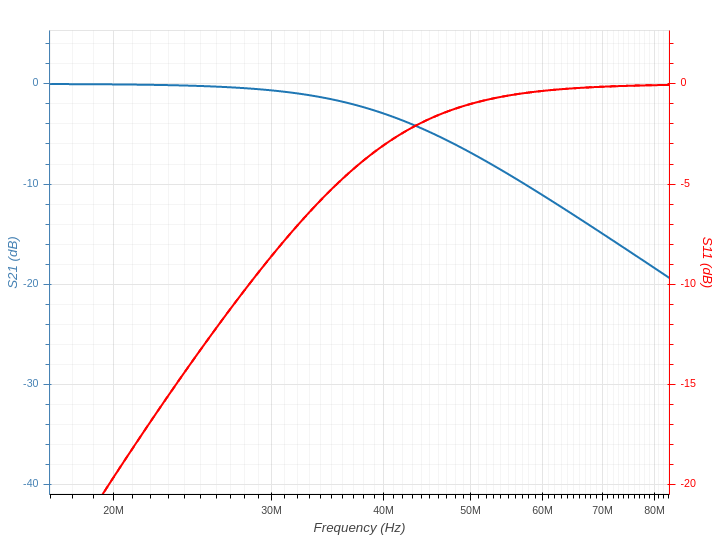
\includegraphics[width=130mm]{./Figures/respFrec.png}
	\caption{Respuesta en frecuencia deseada.}
	\label{fig:respFrec}
\end{figure}


El filtro implementado es un filtro \textit{Butterworth} diferencial de 3er orden con una atenuación de -3dB en 40 MHz, figura \ref{fig:schFiltro}. El ingreso de la señal al filtro se realiza por medio de dos capacitores de desacople y un transformador 1:1, esto permite conectar un sensor inductivo en modo común o diferencial. 

\begin{figure}[ht]
	\centering
	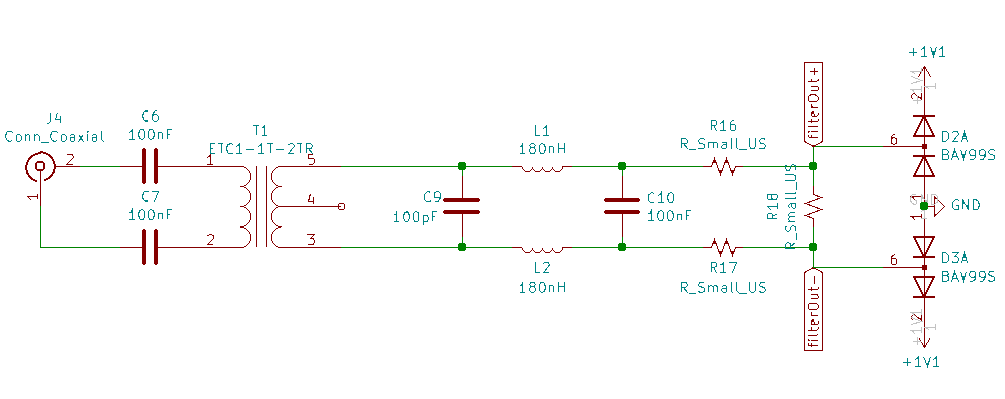
\includegraphics[width=140mm]{./Figures/schFiltro.png}
	\caption{Filtro diferencial \textit{Butterworth} de 3er orden. Frecuencia de corte 40Mhz.}
	\label{fig:schFiltro}
\end{figure}


Puede observarse que al final del filtro se incluye un divisor resistivo y un enclavamiento de diodos para proteger al periférico de sobretensiones. El divisor permite atenuar linealmente la señal en caso de requerir mayor rango dinámico de entrada, también podría servir en caso de requerir agregar una etapa más al filtro.

\subsection{Esquemático general} 

El módulo central es el microprocesador LPC4370, figura \ref{fig:schCentral}. A este llegan la señal analógica proveniente del filtro diferencial y la entrada aislada de la detección del cruce por cero. Puede observarse los componentes necesarios para el funcionamiento reloj de tiempo real (RTC), estos son un cristal de 32 KHz y una batería.


\begin{figure}[ht]
	\centering
	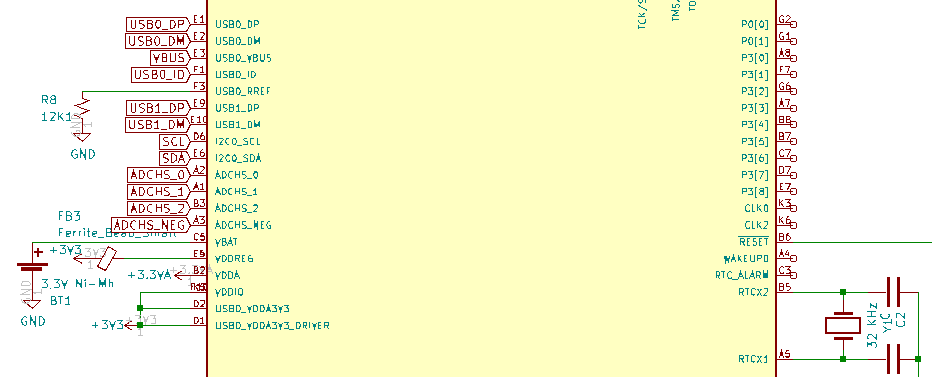
\includegraphics[width=140mm]{./Figures/schCentral.png}
	\caption{Procesador y RTC.}
	\label{fig:schCentral}
\end{figure}


\subsection{Fuente}

La fuente de alimentación, figura \ref{fig:schPwr}, fue diseñada por medio de dos reguladores LDO. Se utilizó el regulador de 3,3 V junto con dos filtros PI para generar dos ramas, una para los módulos digitales y otra los módulos analógicos. El regulador de 1,1 V cumple la función de generar la tensión de enclavamiento para el circuito de protección de la etapa analógica.


\begin{figure}[ht]
	\centering
	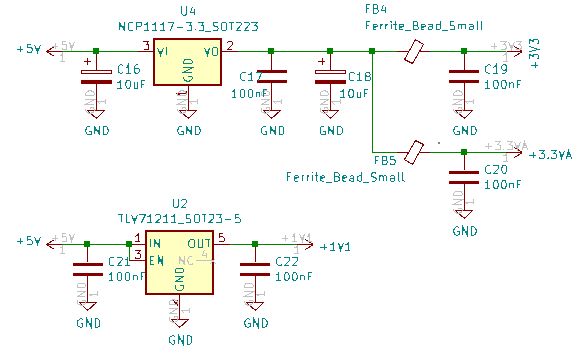
\includegraphics[width=110mm]{./Figures/schPwr.png}
	\caption{Fuentes de alimentación.}
	\label{fig:schPwr}
\end{figure}

\vspace{5mm}

\subsection{Comunicaciones}

Como periféricos de comunicación se proporcionó un puerto 232, figura \ref{fig:schSerial}, para acceder a la interfaz del sistema. 

\begin{figure}[ht]
	\centering
	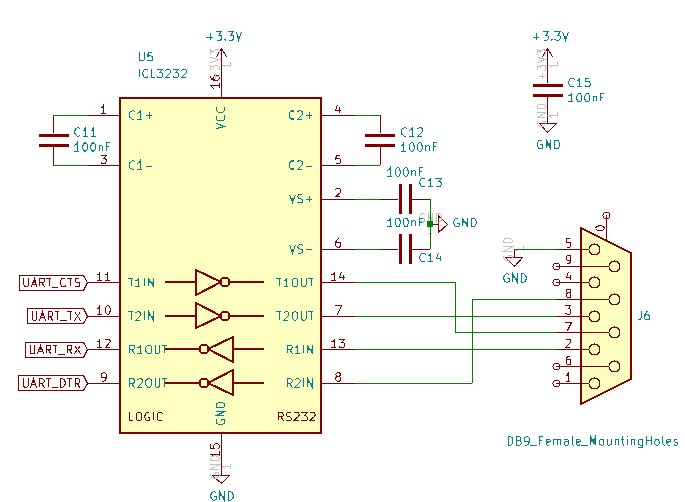
\includegraphics[width=95mm]{./Figures/schSerial.png}
	\caption{Circuito de comunicacion serial.}
	\label{fig:schSerial}
\end{figure}

También se incluyeron dos puertos USB de alta velocidad, figura \ref{fig:schUSB}, uno para conexión directa de un pendrive y otro para conexión \textit{on-the-go} para futuras opciones.

\begin{figure}[ht]
	\centering
	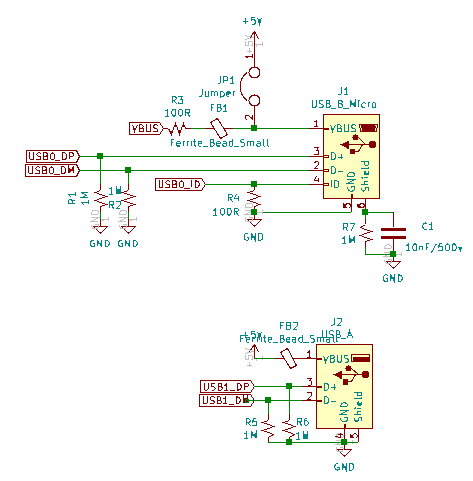
\includegraphics[width=90mm]{./Figures/schUSB.png}
	\caption{Circuitos de comunicacion USB.}
	\label{fig:schUSB}
\end{figure}

\newpage

\section{Diseño del Firmware}

Si bien el LPC4370 dispone de tres núcleos, este trabajo se realizó utilizando solo el cortex M4 dejando libres los dos cortex M0. De esta forma quedan recursos disponibles para implementar futuros procesamientos de la señal. 

Inicialmente se había planificado utilizar un sistema operativo de tiempo real, pero se descartó debido a que la ejecución de tareas durante el proceso de disparo del \textit{trigger} generan \textit{jitter} al comienzo de la adquisición. 

Las soluciones planteadas para este problema fueron:
\vspace{5mm}

\begin{itemize}
\item detener el scheduler en momentos específicos.
\item portar el kernel de freertos tickless para este procesador.
\item evitar el uso de un sistema operativo y realizar el software bajo el patrón de software \textit{superpoll}.
\end{itemize}   

\vspace{5mm}

Por ser una solución de menor complejidad y debido al tiempo disponible para realizar el trabajo, la última alternativa fue la elegida.

El firmware fue desarrolado en lenguaje C y se dividió en varios módulos funcionales que encapsulan su comportamiento, figura \ref{fig:firmBloques}. La interacción entre los módulos se realizó por medio de funciones públicas utilizadas como interfaces. 
\vspace{10mm}

\begin{figure}[ht]
	\centering
	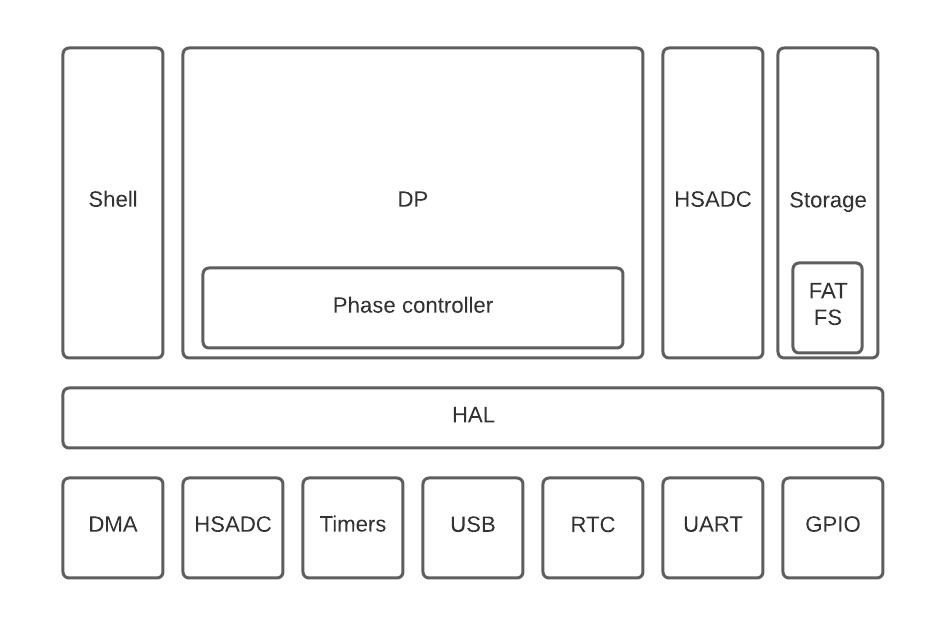
\includegraphics[width=140mm]{./Figures/firmBloques.png}
	\caption{Diagrama en bloques de los módulos de firmware.}
	\label{fig:firmBloques}
\end{figure}


\subsection{Shell}
El equipo dispone de una interfaz de usuario desarrollada para funcionar en cualquier terminal estándar de 80 caracteres por línea, esta es accesible por medio de un puerto serial bajo una configuración 115200,8,n,1.

La interfaz permite configurar el equipo, realizar, navegar y visualizar mediciones. Los comandos se componen de una palabra principal y en algunos casos permiten parámetros adicionales. 

\vspace{5mm}

Existen 4 grupos de comandos:
\begin{itemize}
\item  de configuración.
\item  de navegación.
\item  de visualización.
\item de estado. 

\end{itemize}

\vspace{5mm}

Breve descripción de los comandos:
\begin{itemize}
\item mode -a [m]: permite activar el modo de adquisición automático con un intervalo de tiempo [minutos]. Este modo inicializa la creación de un patrón de DP cada \textit{m} minutos.
\item mode -i [g-p] : Inicializa la creación de un patrón de DP. Con el parámetro [g] lo grafica por medio de caracteres ASCII y no es guardado. Con el parámetro [p] el patrón y el muestreo de las descargas parciales son guardados en el pendrive.
\item mode -d : Desarma el trigger y en caso de haber un patrón de DP en proceso de creación lo guarda.
\item dccal: Calibración para eliminar componente de continua.
\item conf -t [mV] : Permite configurar el valor del trigger en [mV]. El mismo valor será considerado como absoluto y será establecido como trigger positivo y negativo.
\item conf -q [puntos] : Permite configurar la cantidad de puntos (DP) que constituirán un patrón de DP (hasta 1500). 
\item conf -s [muestras] : Permite configurar la cantidad de muestras por DP (hasta 968).
\item time -g : Imprime el valor de fecha y hora en pantalla bajo el formato hh:mm:ss DD/MM/AAAA.
\item time -s [hh:mm:ss DD/MM/AAAA]: Permite configurar la fecha y hora.
\item lspd : Lista todos los patrones de DP existentes en el pendrive.
\item lspd -f [AAAAMMDDhhmm]:  Lista los patrones existentes en el pendrive y los filtra según el año (AAAA), mes (MM), día (DD), horas (hh), minutos (mm) y segundos (ss) ingresados. Cualquier atributo puede reemplazarse por el caracter ‘?’ para ignorar el filtro.
\item dwnpd -g [AAAAMMDDhhmm] : Permite graficar por medio de caracteres ASCII el patrón de descargas parciales seleccionado.
\item dwnpd -t [AAAAMMDDhhmm] : Permite enviar en forma de tabla el patrón seleccionado.
\item restart : Reinicia el cpu
\item info -s : Brinda información sobre el sistema
\item ?: Información sobre los comandos.
\end{itemize}

\vspace{5mm}

La interfaz dispone de un modo de visualización de patrones de descarga parcial generado por caracteres \textit{ascii}, figura \ref{fig:firmInterfaz}. Debido a la baja resolución existente en este modo, se utilizaron diferentes caracteres para representar densidad de DP en un área del patrón determinada. Este modo es especialmente práctico para configuración o consultas remotas. También puede solicitarse que una DP sea visualizada en forma de tabla.

\vspace{5mm}

\begin{figure}[ht]
	\centering
	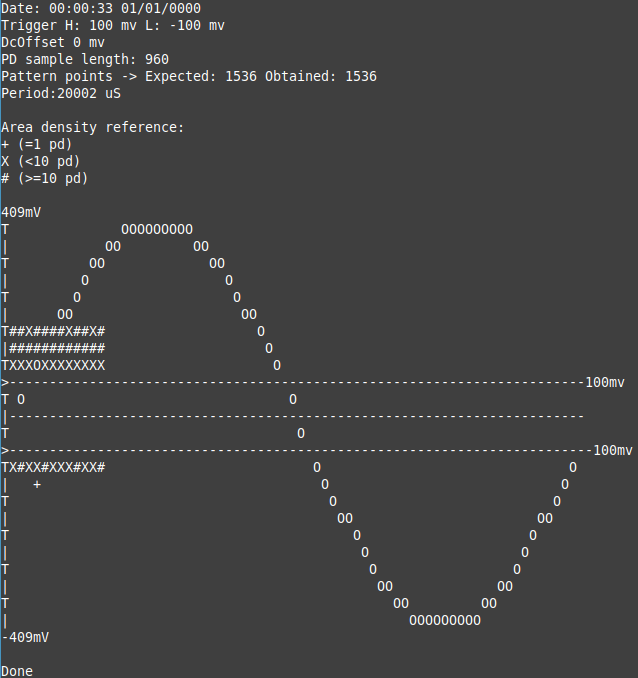
\includegraphics[width=130mm]{./Figures/firmInterfaz.png}
	\caption{Patrón de DP por terminal.}
	\label{fig:firmInterfaz}
\end{figure}

Los archivos almacenados en el pendrive por cada patrón de DP son tres, figura \ref{fig:firmFiles}. Un archivo \enquote{.info} que contiene los parámetros de la medición realizada, un archivo \enquote{.mem} que contiene los datos crudos con las formas de onda de las DP y un archivo \enquote{.csv}. Este último archivo puede ser abierto por cualquier planilla de cálculo y contiene el patrón de DP representado por los conjuntos \enquote{pico-fase}.

\vspace{5mm}

\begin{figure}[ht]
	\centering
	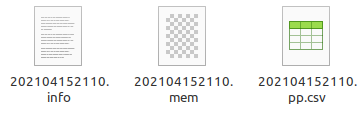
\includegraphics[width=60mm]{./Figures/firmFiles.png}
	\caption{Archivos generados como resultado de la creación de un patrón.}
	\label{fig:firmFiles}
\end{figure}

\subsection{DP}

Dentro de este módulo se realiza el control de las adquisiciones de DP, el posterior procesamiento y conformación del patrón. Este es el módulo central, funciona como consumidor de las funciones que implementan los demás módulos.

Dentro de este módulo tambien se realiza el control de fase. La detección de cruce por cero es realizada por una interrupción por hardware configurada por flanco ascendente. En la rutina de interrupción se inicia un timer que se encarga de medir el tiempo de forma constante entre cruces. Consultando este timer en cualquier momento y desde cualquier parte del código, puede conocerse por regla de tres simple la fase de la senoide de referencia. En la figura \ref{fig:firmFSM} puede verse el diagrama de la máquina de estado encargada de controlar el momento angular.

\begin{figure}[ht]
	\centering
	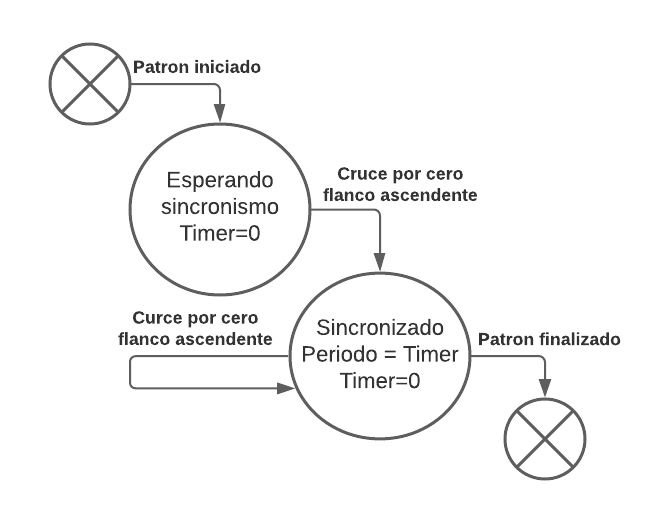
\includegraphics[width=100mm]{./Figures/firmZCFSM.png}
	\caption{FSM control de fase.}
	\label{fig:firmFSM}
\end{figure}

\newpage

\subsection{HSADC}

La gestión de memoria interna fue una pieza clave para el correcto funcionamiento del sistema. El conversor analógico digital junto con su acceso directo a memoria (DMA) generan muestras de 12 bits a una tasa de 80 MHz. Debido a la arquitectura del cortex M4, los accesos al mismo banco de memoria no pueden realizarse de forma simultánea. Para asegurar que no se pierdan muestras de la adquisición, se asignó al periférico ADC un banco de memoria exclusivo, figura \ref{fig:firmMemoria}.

\begin{figure}[ht]
	\centering
	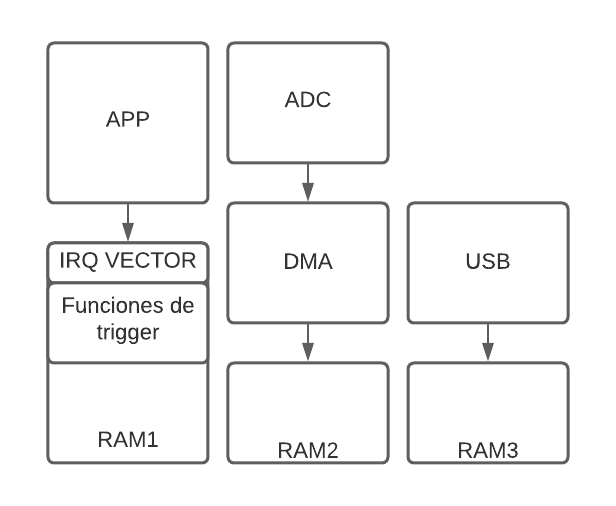
\includegraphics[width=110mm]{./Figures/firmMemoria.png}
	\caption{Diagramas de bloque general de distribución de memoria.}
	\label{fig:firmMemoria}
\end{figure}

Un disparo de \textit{trigger} se realiza por medio de una comparación entre una muestra y un umbral establecido previamente. Para poder realizar esta comparación el periférico necesita adquirir muestras constantemente, esto genera un flujo de datos que debe administrarse. Para resolver esto se utilizó una cola circular en memoria en donde el DMA copia los datos adquiridos de forma constante y elimina siempre la muestra más antigua. Cuando el \textit{trigger} es disparado se almacena el puntero a la posición inicial y cuando la cola completa la vuelta se finaliza la adquisición. El resultado es una ventana de \textit{N} muestras que puede ser propagada a otras capas de software para su correcta manipulación. 

Por practicidad, el modulo de firmware HSADC administra su memoria como un único banco, figura \ref{fig:firmBanco}, este banco a su vez es dividido en \textit{slots}. Todos los slots son de igual tamaño y permiten adquirir ininterrumpidamente a partir de un disparo de trigger. Una vez concluida la adquisición del \textit{slot},  en caso de quedar slots libres el sistema se rearma y queda a la espera de un próximo disparo. En caso de haber completado todos los \textit{slots} del banco de memoria, se procesa y almacena.

\begin{figure}[ht]
	\centering
	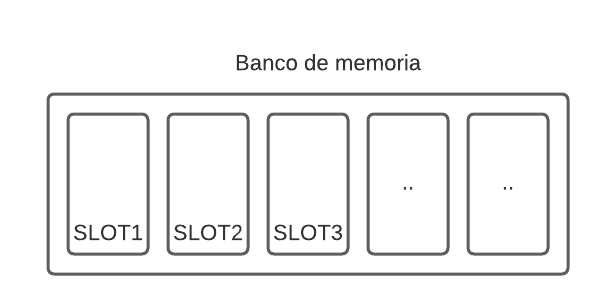
\includegraphics[width=100mm]{./Figures/firmBanco.png}
	\caption{Banco de memoria.}
	\label{fig:firmBanco}
\end{figure}

\newpage

\subsection{Storage}

Este módulo se encarga de encapsular el funcionamiento del pendrive y su sistema de archivos. Implementa el sistema de archivos FAT32 por medio de la librería FatFs \citep{chanWeb:1} combinado con los drivers USB provistos por NXP.


\section{Herramientas de usuario}

Para dar mayor capacidad de análisis sobre las mediciones adquiridas se desarrollaron dos scripts en Python3 que procesan los datos almacenados en el pendrive. 
\begin{itemize}
\item El primero permite generar un patrón de DP de forma gráfica a partir de una archivo \enquote{.csv}.
\item El segundo permite reconstruir las señales obtenidas de cada DP a partir de una archivo \enquote{.mem} y generar un gráfico por cada una.
\end{itemize}  

\vspace{5mm}

\begin{figure}[ht]
	\centering
	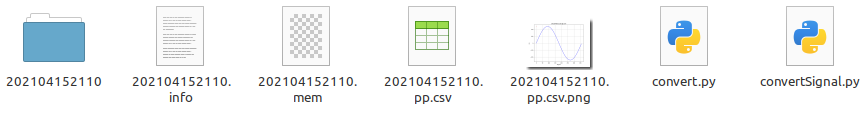
\includegraphics[width=140mm]{./Figures/firmAllFiles.png}
	\caption{Árbol completo de archivos luego del procesamiento con scripts.}
	\label{fig:firmAllFiles}
\end{figure}

\section{Prototipo funcional}

Un prototipo funcional fue montado como validador tecnológico y a su vez para poder llevar a cabo los ensayos. El mismo fue construido utilizando una placa de desarrollo \enquote{LPC link2}, figura \ref{fig:hardLPC}. A pesar de no estar disponibles todos los pines del microprocesador la placa fue modificada para poder acceder a todos los periféricos requeridos en este trabajo. La única restricción encontrada fue el acceso a la alimentación independiente del reloj de tiempo real lo cual hace que, en este prototipo, la fecha y hora se pierda siempre que falte el suministro eléctrico. 

\begin{figure}[ht]
	\centering
	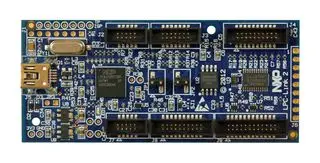
\includegraphics[width=90mm]{./Figures/hardLPC.png}
	\caption{LPC link2.}
	\label{fig:hardLPC}
\end{figure}

\vspace{10mm}

Como tareas de modificación se removieron los filtros existentes en modo común de las entradas analogicas, para que no afecten a los nuevos filtros diferenciales conectados. Tambien se agregó un cristal de 32 Khz como oscilador del reloj de tiempo real.

La placa de desarrollo solo dispone de un puerto USB diseñado para ser utilizado como device y ser conectado a la PC. El circuito fue modificado para funcionar como host y ser alimentado desde la fuente. También se utilizó un adaptador micro USB a USB A para poder conectar un pendrive.  

Para finalizar el prototipo funcional, figura \ref{fig:hardProto}, se agregó una placa adicional con el filtro diferencial y la etapa de optoacoplado. La conexiones entre los dos circuitos impresos fueron realizadas por medio de los puertos de expansión del LPC link2. 

\begin{figure}[ht]
	\centering
	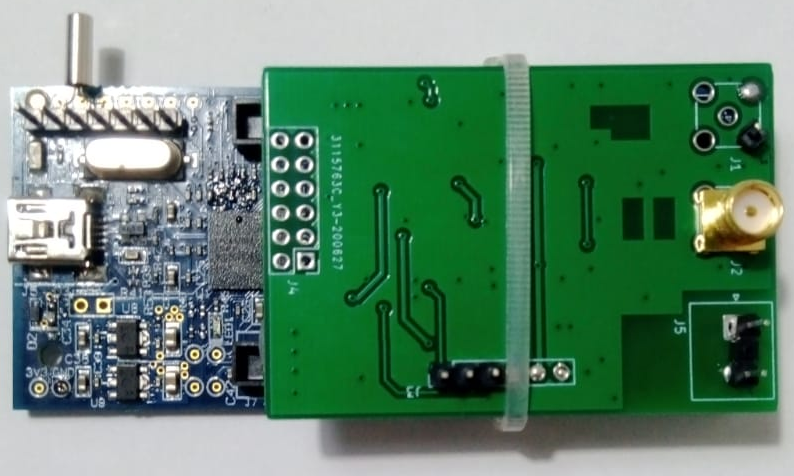
\includegraphics[width=80mm]{./Figures/hardProto.png}
	\caption{Prototipo funcional.}
	\label{fig:hardProto}
\end{figure}
% Chapter Template

\chapter{Ensayos y resultados} % Main chapter title

\label{Chapter4} % Change X to a consecutive number; for referencing this chapter elsewhere, use \ref{ChapterX}

%----------------------------------------------------------------------------------------
%	SECTION 1
%----------------------------------------------------------------------------------------

\section{Banco de pruebas}

\section{Ensayos de amplitud}

\section{Ensayos de disparo}

\section{Ensayos de fase}

\section{Tiempos de procesamiento y almacenado}

\section{Pruebas en campo}
 
% Chapter Template

\chapter{Conclusiones} % Main chapter title

\label{Chapter5} % Change X to a consecutive number; for referencing this chapter elsewhere, use \ref{ChapterX}
Durante este capítulo se realiza un breve resumen del trabajo realizado, los problemas encontrados y los resultados obtenidos. También se incluye una reseña de posibles implementaciones futuras.
%----------------------------------------------------------------------------------------
%	SECTION 1
%----------------------------------------------------------------------------------------

\section{Trabajo obtenido}

El trabajo finalizó con el desarrollo exitoso de un prototipo medidor de descargas parciales. Este se armó utilizando una placa de desarrollo “LPC Link 2” y un breakout para el filtrado de la señal analogica y adquisición de la senoide de referencia. El equipo logrado es de bajo costo, tamaño reducido y cumple con todos los requerimientos pautados con el cliente a excepción de los requerimientos Req 23 y Req 24 que fueron modificados sin perjudicar la funcionalidad del equipo.

Este prototipo es capaz de generar un patrón de descargas parciales de forma autónoma y almacenarlo en un pendrive USB. Para esto permite configurar una serie de parámetros que luego serán utilizados en la adquisición del patrón. Además de realizar un patrón de descargas parciales el equipo permite, de forma optativa, almacenar el muestreo completo de cada descarga parcial. Los datos obtenidos pueden ser accedidos por medio del puerto serie usando la interfaz de usuario implementada o pueden procesarse desde la unidad flash utilizado una serie de scripts provistos realizados en Python.

Por medio de las pruebas realizadas pudo validarse la correcta medición de descargas parciales sintetizadas de forma digital, también se validó la correcta confección del patrón de descargas parciales. Debido a la pandemia global causada por el COVID-19 no fue posible realizar pruebas en el laboratorio de la Universidad Tecnológica Nacional Regional General Pacheco.

En cuanto a la planificación se cumplio dentro de los plazos esperados a pesar de haberse manifestado el principal riesgo: “restricciones de velocidad para realizar la adquisición”. Se invirtió una suma de tiempo sustancial en mitigar este riesgo, durante esta etapa se intentó resolver la adquisición por medio de un FPGA y un conversor externo de alta velocidad de forma exitosa. Finalmente fue reemplazado por el LPC4370 por motivos de costo y complejidad.

%----------------------------------------------------------------------------------------
%	SECTION 2
%----------------------------------------------------------------------------------------
\section{Conocimientos aplicados}

Durante la realización de este proyecto se aplicaron conocimientos adquiridos en el transcurso de la especialidad. Las asignaturas que más aportaron para la realización de este trabajo fueron:
\begin{itemize}
\item Gestión de proyecto para crear la documentación relativa a la planificación y seguimiento.
\item Programación de microcontroladores para la implementación del firmware en C del microcontrolador ARM M4 elegido.
\item Ingeniería de software para seguir buenas prácticas de diseño y documentación.
\end{itemize}

\section{Trabajo futuro}
A fin de lograr un equipo apto para el mercado como actividades de mejora a futuro se propone:
\begin{itemize}
\item Utilizar los dos cortex M0 para revertir los efectos del filtro de forma digital y hacer un resampling de la señal con el objetivos de mejorar la precisión del máximo obtenido.
\item Permitir la carga de parámetros de configuración por medio del pendrive USB. 
\item Implementar un sistema de pre-trigger que permita mantener n muestras posteriores al momento del disparo.
\end{itemize}
 

%----------------------------------------------------------------------------------------
%	CONTENIDO DE LA MEMORIA  - APÉNDICES
%----------------------------------------------------------------------------------------

\appendix % indicativo para indicarle a LaTeX los siguientes "capítulos" son apéndices

% Incluir los apéndices de la memoria como archivos separadas desde la carpeta Appendices
% Descomentar las líneas a medida que se escriben los apéndices

%\include{Appendices/AppendixA}
%\include{Appendices/AppendixB}
%\include{Appendices/AppendixC}

%----------------------------------------------------------------------------------------
%	BIBLIOGRAPHY
%----------------------------------------------------------------------------------------

\Urlmuskip=0mu plus 1mu\relax
\raggedright
\printbibliography[heading=bibintoc]

%----------------------------------------------------------------------------------------

\end{document}  
